% 原书印刷184–188页，PDF物理215–219页；图见物理220页.
\subsection{次序统计量}\label{sec:5.4}
随机样本中的最小、最大或中间观测值等，可以提供额外的概要信息.例如，为未来紧急情况制定计划时，过去50年记录到的最高洪水水位或最低冬季气温可能是有用的数据.上个月出售房屋的价格中位数可能有助于估计生活成本.这些都是次序统计量（order statistics）的例子.
\begin{definition}\label{def:5.4.1}\index{SI0731@次序统计量}
随机样本$X_1,\ldots,X_n$的次序统计量，是将样本值按递增次序排列后所得的值，记为$X_{(1)},\ldots,X_{(n)}$.
\end{definition}
次序统计量是满足$X_{(1)}\le\cdots\le X_{(n)}$的随机变量.特别地，
$$\begin{aligned}
X_{(1)}&=\min_{1\le i\le n}X_i,\\
X_{(2)}&=\text{第二小的$X_i$},\\
&\ \vdots\\
X_{(n)}&=\max_{1\le i\le n}X_i.
\end{aligned}$$
既然它们是随机变量，就可讨论它们取各种值的概率.计算这些概率需要次序统计量的pdf或pmf.连续总体随机样本的次序统计量pdf公式是本节后面的主要内容，但先介绍几种易于用次序统计量定义的统计量.

样本极差（sample range）\index{SI0933@极差}\semanticindexanchor{933:215}$R=X_{(n)}-X_{(1)}$是最小观测值与最大观测值之间的距离.它衡量样本的离散程度，应反映总体的离散程度.

样本中位数（sample median）记为$M$，大约一半的观测小于$M$，另一半大于$M$.用次序统计量定义为
\begin{equation}\label{eq:5.4.1}\index{SI0930@中位数}
M=\begin{cases}X_{((n+1)/2)},&n\text{为奇数},\\[2pt]
\bigl(X_{(n/2)}+X_{(n/2+1)}\bigr)/2,&n\text{为偶数}.
\end{cases}
\end{equation}
中位数是一种位置度量，可以作为样本均值的替代量.样本中位数相对于样本均值的一个优点，是它受极端观测值的影响较小（详见\autoref{sec:10.2}）.

虽然均值与中位数有关，但它们通常衡量不同的东西.例如，最近一次棒球薪资谈判的主要争议点，是老板对球员养老金的缴款.老板的观点可以概括为：“棒球运动员的平均年薪为433,659美元；有这么多钱，现有养老金已经足够.”但球员的观点是：“超过一半的球员年收入不到250,000美元，而且多数球员的职业生涯短暂，需要较高养老金提供保障.”（这些数字属于1988赛季，而非发生争议的年份.）双方的数字都正确，但老板讨论的是均值，而球员讨论的是中位数.
\sourcepageanchor{216}
大约十来位年薪超过200万美元的球员，就能把平均薪资抬到433,659美元，而大多数球员收入不到250,000美元，包括所有年薪62,500美元的新秀.讨论工资、价格或任何有少数极端值的变量时，中位数比均值更能代表“典型”值.还有其他可由次序统计量定义、对极端值较不敏感的统计量，例如\autoref{exercise:10.20}中的$\alpha$截尾均值；\hyperref[bib:source318]{Tukey（1977）}等书对此有所讨论.

对0与1之间任意数$p$，第$100p$样本百分位数（sample percentile）\index{SI0754@百分位数}\semanticindexanchor{754:216}是这样一个观测值：大约$np$个观测值比它小，$n(1-p)$个比它大.第50样本百分位数（$p=.5$）就是样本中位数.对于其他$p$值，可按下述方式用次序统计量更精确地定义样本百分位数.
\begin{definition}\label{def:5.4.2}
出现在下标中的记号$\{b\}$，表示将$b$按通常方法舍入到最近的整数.更精确地，若$i$为整数且$i-.5\le b<i+.5$，则$\{b\}=i$.
\end{definition}
当$1/(2n)<p<.5$时，第$100p$样本百分位数是$X_{(\{np\})}$；当$.5<p<1-1/(2n)$时，则是$X_{(n+1-\{n(1-p)\})}$.例如，若$n=12$，要求第65百分位数，注意$12\times(1-.65)=4.2$，且$12+1-4=9$，所以它是$X_{(9)}$.对$p$的范围有限制，是因为样本容量限制了样本百分位数的范围.

将$p<.5$与$p>.5$两种情形分别定义，是为了让样本百分位数具有如下对称性：若第$100p$样本百分位数为第$i$小的观测值，则第$100(1-p)$样本百分位数应为第$i$大的观测值，上述定义正好满足这一点.例如，$n=11$时，第30样本百分位数为$X_{(3)}$，第70样本百分位数为$X_{(9)}$.

除了中位数，还常用两个样本百分位数：\index{SI0860@四分位数}\semanticindexanchor{860:216}下四分位数（lower quartile，第25百分位数）与上四分位数（upper quartile，第75百分位数）.有时用四分位距（interquartile range），即上、下四分位数之间的距离，衡量离散程度.

由于次序统计量是样本的函数，关于次序统计量的概率可由样本的概率计算.若$X_1,\ldots,X_n$为iid离散随机变量，计算次序统计量的概率主要是一个计数问题.\autoref{thm:5.4.3}推导了相应公式.若$X_1,\ldots,X_n$为来自连续总体的随机样本，\autoref{thm:5.4.4}和\autoref{thm:5.4.6}给出一个或多个次序统计量pdf的方便表达式，之后可用来推导次序统计量的函数的分布.
\begin{theorem}\label{thm:5.4.3}\index{SI0732@累积分布函数}\index{SI0736@概率质量函数}
设$X_1,\ldots,X_n$为来自pmf为$f_X(x_i)=p_i$的离散分布的随机样本，其中$x_1<x_2<\cdots$是$X$按递增顺序排列的可能取值.定义
$$\begin{aligned}P_0&=0,\\P_1&=p_1,\\P_2&=p_1+p_2,\\&\ \vdots\\P_i&=p_1+p_2+\cdots+p_i,\\&\ \vdots\end{aligned}$$
以$X_{(1)},\ldots,X_{(n)}$表示样本的次序统计量.则
\begin{equation}\label{eq:5.4.2}
P(X_{(j)}\le x_i)=\sum_{k=j}^n\binom nk P_i^k(1-P_i)^{n-k}
\end{equation}
并且
\begin{equation}\label{eq:5.4.3}
P(X_{(j)}=x_i)=\sum_{k=j}^n\binom nk\left[P_i^k(1-P_i)^{n-k}-P_{i-1}^k(1-P_{i-1})^{n-k}\right].
\end{equation}
\end{theorem}
\sourcepageanchor{217}
\begin{proof}
固定$i$，令随机变量$Y$表示$X_1,\ldots,X_n$中小于或等于$x_i$的个数.对于每个$X_j$，将事件$\{X_j\le x_i\}$称为“成功”，$\{X_j>x_i\}$称为“失败”.则$Y$是$n$次试验的成功次数.由于$X_1,\ldots,X_n$同分布，每次试验的成功概率相同，都是$P_i=P(X_j\le x_i)$.由于$X_j$与其他$X_i$独立，第$j$次试验成功还是失败与其他试验结果独立.故$Y\sim\operatorname{binomial}(n,P_i)$.

事件$\{X_{(j)}\le x_i\}$等价于$\{Y\ge j\}$，即至少$j$个样本值不超过$x_i$.\eqref{eq:5.4.2}表示这一二项概率：
$$P(X_{(j)}\le x_i)=P(Y\ge j).$$
\eqref{eq:5.4.3}只不过表示下面的差：
$$P(X_{(j)}=x_i)=P(X_{(j)}\le x_i)-P(X_{(j)}\le x_{i-1}).$$
$i=1$是一个例外，此时$P(X_{(j)}=x_1)=P(X_{(j)}\le x_1)$.定义$P_0=0$使\eqref{eq:5.4.3}也包含这个例外.
\end{proof}
若$X_1,\ldots,X_n$为来自连续总体的随机样本，情形会稍简单，因为任意两个$X_j$相等的概率为0，无须担心并列值.故$P(X_{(1)}<X_{(2)}<\cdots<X_{(n)})=1$，且$(X_{(1)},\ldots,X_{(n)})$的样本空间为$\{(x_1,\ldots,x_n):x_1<x_2<\cdots<x_n\}$.\autoref{thm:5.4.4}和\autoref{thm:5.4.6}再次利用二项分布论证，分别给出单个次序统计量的pdf和两个次序统计量的联合pdf.
\begin{theorem}\label{thm:5.4.4}\index{SI0735@概率密度函数}
设$X_{(1)},\ldots,X_{(n)}$是随机样本$X_1,\ldots,X_n$的次序统计量，总体连续且cdf为$F_X(x)$、pdf为$f_X(x)$.则$X_{(j)}$的pdf为
\begin{equation}\label{eq:5.4.4}
f_{X_{(j)}}(x)=\frac{n!}{(j-1)!(n-j)!}f_X(x)[F_X(x)]^{j-1}[1-F_X(x)]^{n-j}.
\end{equation}
\end{theorem}
\begin{proof}
先求$X_{(j)}$的cdf，再求导得到pdf.如\autoref{thm:5.4.3}，令$Y$表示$X_1,\ldots,X_n$中不超过$x$的个数.把事件$\{X_j\le x\}$定义为“成功”，可知$Y\sim\operatorname{binomial}(n,F_X(x))$.（注意，\autoref{thm:5.4.3}中可写$P_i=F_X(x_i)$.另外，虽然$X_1,\ldots,X_n$是连续随机变量，计数变量$Y$却是离散的.）因此
$$F_{X_{(j)}}(x)=P(Y\ge j)=\sum_{k=j}^n\binom nk[F_X(x)]^k[1-F_X(x)]^{n-k},$$
而$X_{(j)}$的pdf为
\begin{align*}
f_{X_{(j)}}(x)&=\frac d{dx}F_{X_{(j)}}(x)\\
&=\sum_{k=j}^n\binom nk\Bigl(k[F_X(x)]^{k-1}[1-F_X(x)]^{n-k}f_X(x)\\
&\hspace{38mm}-(n-k)[F_X(x)]^k[1-F_X(x)]^{n-k-1}f_X(x)\Bigr)\quad\text{（链式法则）}\\
&=\binom nj j f_X(x)[F_X(x)]^{j-1}[1-F_X(x)]^{n-j}\\
&\quad+\sum_{k=j+1}^n\binom nk k[F_X(x)]^{k-1}[1-F_X(x)]^{n-k}f_X(x)\\
&\quad-\sum_{k=j}^{n-1}\binom nk(n-k)[F_X(x)]^k[1-F_X(x)]^{n-k-1}f_X(x),
\end{align*}
最后一项求和中$k=n$的项为零.
\sourcepageanchor{218}
改变求和指标，继续得到
\begin{align*}
f_{X_{(j)}}(x)&=\frac{n!}{(j-1)!(n-j)!}f_X(x)[F_X(x)]^{j-1}[1-F_X(x)]^{n-j}\\
&\quad+\sum_{k=j}^{n-1}\binom n{k+1}(k+1)[F_X(x)]^k[1-F_X(x)]^{n-k-1}f_X(x)\\
&\quad-\sum_{k=j}^{n-1}\binom nk(n-k)[F_X(x)]^k[1-F_X(x)]^{n-k-1}f_X(x).
\end{align*}
注意
\begin{equation}\label{eq:5.4.5}
\binom n{k+1}(k+1)=\frac{n!}{k!(n-k-1)!}=\binom nk(n-k),
\end{equation}
可见上面最后两个和相消.因此pdf $f_{X_{(j)}}(x)$就是\eqref{eq:5.4.4}的表达式.
\end{proof}
\begin{example}[均匀分布次序统计量的pdf]\label{ex:5.4.5}\index{SI0389@次序统计量}
设$X_1,\ldots,X_n$为iid $\operatorname{uniform}(0,1)$，故$x\in(0,1)$时$f_X(x)=1$、$F_X(x)=x$.由\eqref{eq:5.4.4}，第$j$个次序统计量的pdf为
\begin{align*}
f_{X_{(j)}}(x)&=\frac{n!}{(j-1)!(n-j)!}x^{j-1}(1-x)^{n-j},\qquad x\in(0,1)\\
&=\frac{\Gamma(n+1)}{\Gamma(j)\Gamma(n-j+1)}x^{j-1}(1-x)^{(n-j+1)-1}.
\end{align*}
所以，$\operatorname{uniform}(0,1)$样本的第$j$个次序统计量服从$\operatorname{beta}(j,n-j+1)$分布.由此推得
$$EX_{(j)}=\frac j{n+1},\qquad\operatorname{Var}X_{(j)}=\frac{j(n-j+1)}{(n+1)^2(n+2)}.$$
\end{example}
两个或多个次序统计量的联合分布，可用于推导本节开头提到的某些统计量的分布.任意两个次序统计量的联合pdf由下述定理给出，证明留在\autoref{exercise:5.26}中.
\begin{theorem}\label{thm:5.4.6}\index{SI0734@联合概率密度函数}
设$X_{(1)},\ldots,X_{(n)}$是随机样本$X_1,\ldots,X_n$的次序统计量，总体连续且cdf为$F_X(x)$、pdf为$f_X(x)$.则$X_{(i)}$与$X_{(j)}$（$1\le i<j\le n$）的联合pdf为
\begin{equation}\label{eq:5.4.6}
\begin{aligned}
f_{X_{(i)},X_{(j)}}(u,v)&=\frac{n!}{(i-1)!(j-1-i)!(n-j)!}f_X(u)f_X(v)[F_X(u)]^{i-1}\\
&\quad\times[F_X(v)-F_X(u)]^{j-1-i}[1-F_X(v)]^{n-j},
\end{aligned}
\end{equation}
其中$-\infty<u<v<\infty$.
\end{theorem}
用类似但更繁复的论证，可以推导三个或更多次序统计量的联合pdf.另一个最有用的pdf或许是全体次序统计量的联合pdf $f_{X_{(1)},\ldots,X_{(n)}}(x_1,\ldots,x_n)$，它为
$$f_{X_{(1)},\ldots,X_{(n)}}(x_1,\ldots,x_n)=\begin{cases}
n!f_X(x_1)\cdots f_X(x_n),&-\infty<x_1<\cdots<x_n<\infty,\\
0,&\text{其他情形}.
\end{cases}$$
公式中自然出现$n!$，因为对于任意一组数值$x_1,\ldots,x_n$，将它们分配给$X_1,\ldots,X_n$共有$n!$种等可能方式，且都产生相同的次序统计量值.结合这个联合pdf与\autoref{sec:4}的方法，可以推导边际分布、条件分布以及次序统计量其他函数的分布（见\autoref{exercise:5.27}和\autoref{exercise:5.28}\mbox{）.}
\sourcepageanchor{219}
现在利用联合pdf \eqref{eq:5.4.6}推导本节开头提到的某些函数的分布.
\begin{example}[中程数与极差的分布]\label{ex:5.4.7}\index{SI0931@中程数}\index{SI0945@均匀}
设$X_1,\ldots,X_n$为iid $\operatorname{uniform}(0,a)$，次序统计量为$X_{(1)},\ldots,X_{(n)}$.前面已定义极差$R=X_{(n)}-X_{(1)}$.中程数（midrange）与样本中位数或均值一样，是位置度量，定义为$V=(X_{(1)}+X_{(n)})/2$.我们由$X_{(1)}$与$X_{(n)}$的联合pdf推导$R$与$V$的联合pdf.由\eqref{eq:5.4.6}有
\begin{align*}
f_{X_{(1)},X_{(n)}}(x_1,x_n)&=\frac{n(n-1)}{a^2}\left(\frac{x_n}a-\frac{x_1}a\right)^{n-2}\\
&=\frac{n(n-1)(x_n-x_1)^{n-2}}{a^n},\qquad0<x_1<x_n<a.
\end{align*}
解出$X_{(1)}$和$X_{(n)}$，得$X_{(1)}=V-R/2$、$X_{(n)}=V+R/2$.此变换的Jacobian为$-1$.从$(X_{(1)},X_{(n)})$到$(R,V)$的变换把$\{(x_1,x_n):0<x_1<x_n<a\}$映到$\{(r,v):0<r<a,r/2<v<a-r/2\}$.这是因为显然$0<r<a$，而固定$r$时，$v$从$r/2$（对应$x_1=0,x_n=r$）到$a-r/2$（对应$x_1=a-r,x_n=a$）变化.因此$(R,V)$的联合pdf为
$$f_{R,V}(r,v)=\frac{n(n-1)r^{n-2}}{a^n},\qquad0<r<a,\quad r/2<v<a-r/2.$$
于是$R$的边际pdf为
\begin{equation}\label{eq:5.4.7}
\begin{aligned}
f_R(r)&=\int_{r/2}^{a-r/2}\frac{n(n-1)r^{n-2}}{a^n}\,dv\\
&=\frac{n(n-1)r^{n-2}(a-r)}{a^n},\qquad0<r<a.
\end{aligned}
\end{equation}
当$a=1$时，$r$服从$\operatorname{beta}(n-1,2)$分布.或者，对任意$a$，容易从\eqref{eq:5.4.7}推出$R/a$服从beta分布.注意常数$a$是尺度参数.

$f_{R,V}(r,v)>0$的区域如\autoref{fig:5.4.1}所示，可见$r$的积分范围取决于$v>a/2$还是$v\le a/2$.因此$V$的边际pdf为
$$f_V(v)=\int_0^{2v}\frac{n(n-1)r^{n-2}}{a^n}\,dr=\frac{n(2v)^{n-1}}{a^n},\qquad0<v\le a/2,$$
以及
$$f_V(v)=\int_0^{2(a-v)}\frac{n(n-1)r^{n-2}}{a^n}\,dr=\frac{n[2(a-v)]^{n-1}}{a^n},\qquad a/2<v\le a.$$
这个pdf关于$a/2$对称，并在$a/2$处达到峰值.
\end{example}
\begin{figure}[htbp]\centering
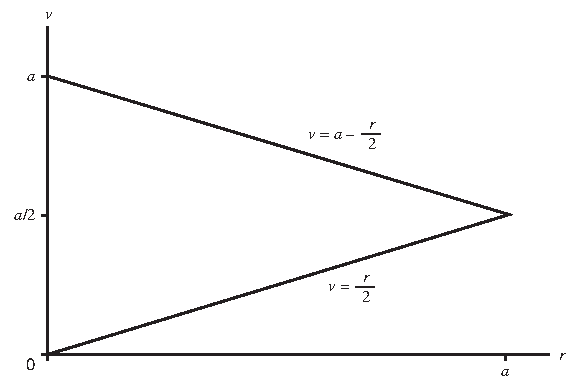
\includegraphics[width=.62\textwidth]{assets/chapter5/fig-5-4-1.pdf}
\caption{\autoref{ex:5.4.7}中$f_{R,V}(r,v)>0$的区域}\label{fig:5.4.1}
\end{figure}
